\newpage

\section{Требования к правилам обмена с системой 1С:УПП.}
\label{sec:exchange}

%Схема обмена по передаче параметров для планирования между 1С:УПП и СИСТЕМОЙ представлена на рисунке \ref{pic:exchange}.
%
%
%\subsection{Справочник ''Номенклатура''}
%
%\subsection{Обмен документом ''Установка цен номенклатуры''}
%






\subsection{Функциональные требования}

\subsubsection{Первоначальная выгрузка}


Необходимо организовать первоначальную выгрузку справочников из 1С:УПП в СИСТЕМУ.
% На Предприятии учет реализован в нескольких информационных базах 1С: Бухгалтерия.

%В последующем необходимо по расписанию выгружать эти справочники из 1С:УПП в Гофротару.

%Справочник <<Типы цен>> передаваться между системами не должен. 

\begin{itemize}
   \item Номенклатура --- загрузить из справочника ''Номенклатура'' согласно правил обмена;
  \item Контрагент --- загрузить полностью из справочника ''Контрагент'';
  \item Договоры контрагентов --- загрузить полностью из справочника ''Договоры контрагентов'';
%   \item Причины брака --- загрузить полностью из справочника  ''Причины брака''.
%   \item Причины остановов --- загрузить полностью из справочника  ''Причины остановов''.
% \item Спецификации номенклатуры --- загрузить согласно правил обмена.

%   \item Единицы измерения --- загрузить полностью из справочника ''Единицы измерения'';
%   \item Ставки НДС --- загрузить полностью из справочника ''Ставки НДС'';
%   \item Структурные единицы --- загрузить полностью из справочника ''Места хранения'';
%   \item Организации --- загрузить полностью из справочника ''Организации'';
%   \item Банки --- загрузить полностью из справочника ''Банки'';
 % \item Сотрудники --- загрузить полностью из справочника ''Банковские счета''.
 \item Физические лица --- загрузить полностью из справочника ''Физические лица''.
% \item Технологические карты --- загрузка полностью из справочника ''Номенклатура'' и ''Характеристика номенклатуры''.
\end{itemize}




  % Первоначальная загрузка справочника ''Номенклатура'' должна быть выполнена по следующему отбору.
% % Table generated by Excel2LaTeX from sheet '1С'
% \scriptsize
% \begin{longtable}{|p{20mm}|p{70mm}|p{64mm}|}
% \hline
% {\bf \parbox[c][15mm]{20mm}{\centeringКод группы}} & {\bf \parbox[c]{70mm}{\centeringПуть}} & \parbox[c]{64mm}{\centeringМатериалы (справочно)} \\
% \hline
% \parbox[c][5mm]{30mm}{00000000067} & Номенклатура-Материалы-Сырье и материалы (10-1) & сырье (бумага, картон) \\
% \hline
% \parbox[c][30mm]{30mm}{00000002884} & Номенклатура-Материалы-Прочие материалы-Сопутствующие & крахмал, едкий натр, бура
% прочие хим.добавки
% клей ПВА
% ленты ПП и ПЭ, скобы, скотч
% стрейч-пленка \\
% \hline
% \parbox[c][9mm]{30mm}{БП-00000989} & Номенклатура-Материалы-Прочие материалы-Покупной гофрокартон & покупной гофрокартон \\
% \hline
% \parbox[c][9mm]{30mm}{00000002632} & Номенклатура-Материалы-Прочие материалы-Флексоформы & оснастка (штанцевые и печатные формы) \\
% \hline
% \parbox[c][5mm]{30mm}{БП-00000996} & Номенклатура-Материалы-Прочие материалы-Краска & флексо-краска \\
% \hline
% \caption{Отбор справочника ''Номенклатура'' для первоначальной загрузки}\label{taB:nomload}
% \end{longtable}  
% \normalsize



\subsubsection{Регулярный обмен}
\label{exchange:regular}
Регулярный обмен между системами 1С: УПП и OPTI-CORRUGATED должен быть настроен по регламентному заданию. Время и периодичность выполнения должны быть заданы в обеих базах.

Механизм обмена - Web-сервис, План обмена.

При обмене с системой 1С: УПП загруженные документы не должны проводиться.

Структура обмена по учету производства представлена на рис. \ref{pic:DFD}.

\begin{figure}[htb]
\begin{center}
   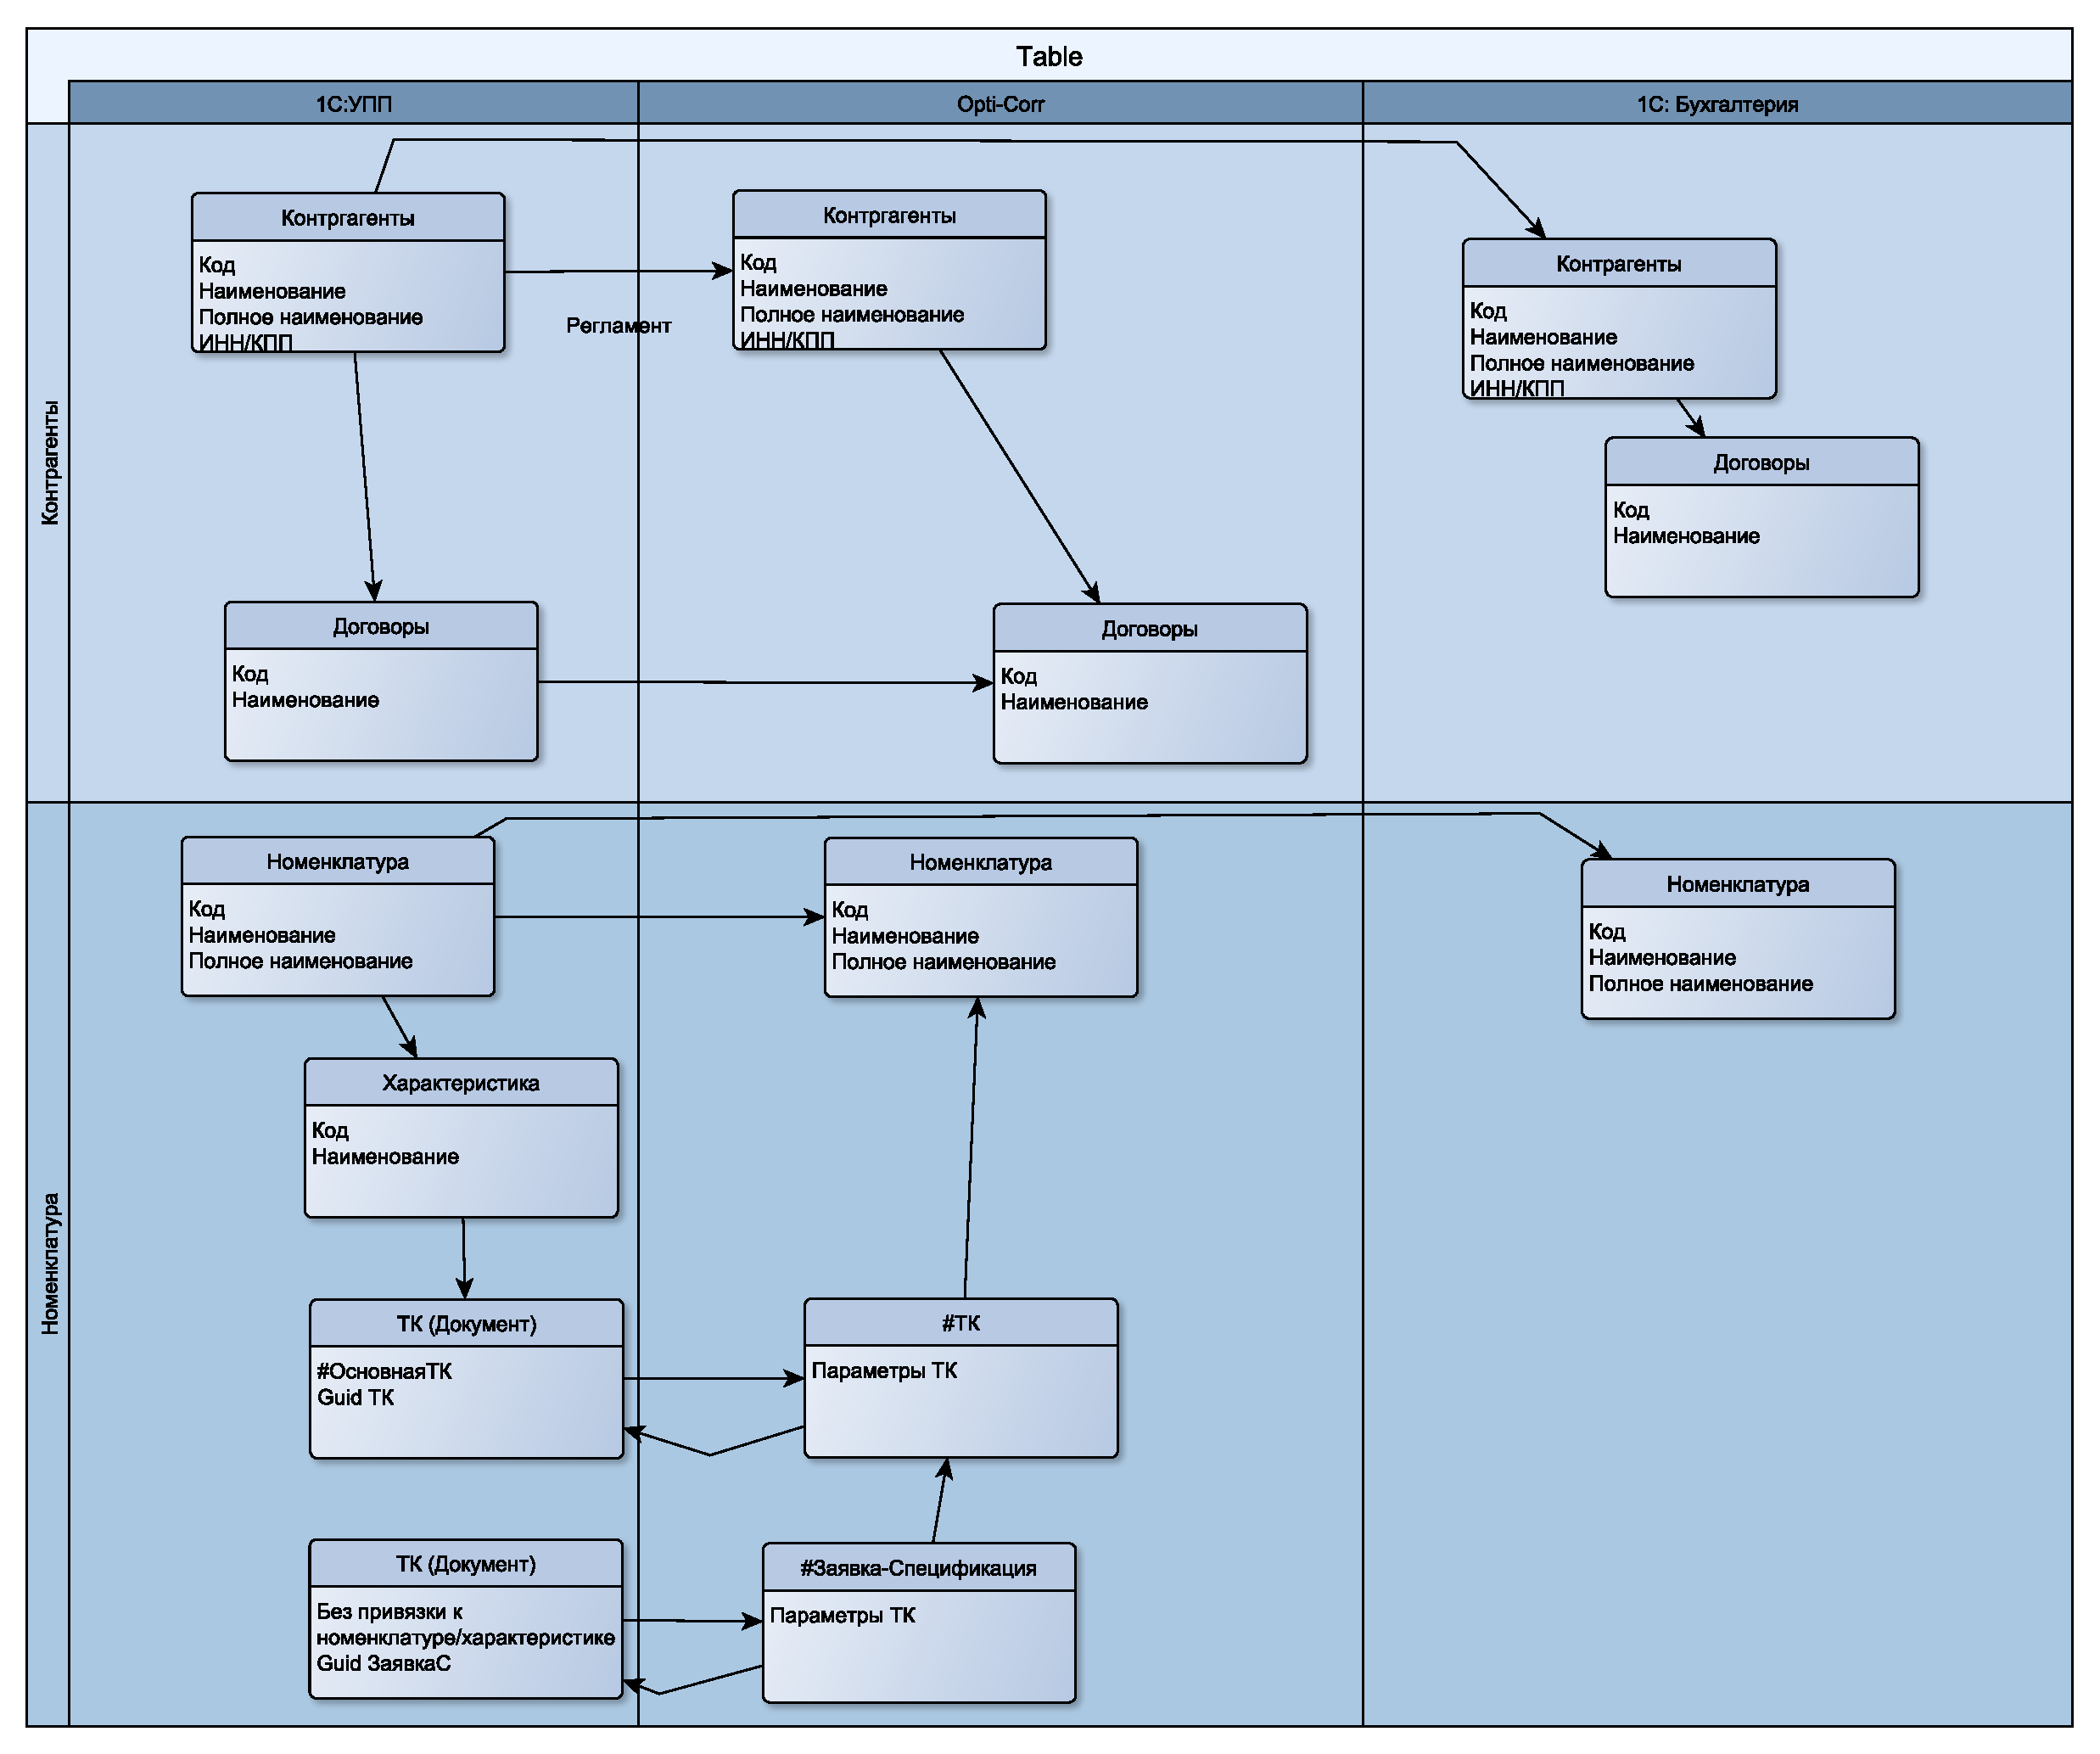
\includegraphics[height=0.8\textheight, width=1\textwidth, angle=0,  keepaspectratio]{50_Pics/DFD.pdf}
\end{center}
   \caption{Потоки обмена информацией между системами. НСИ}
   \label{pic:DFD}
\end{figure}
\FloatBarrier

\begin{figure}[htb]
\begin{center}
  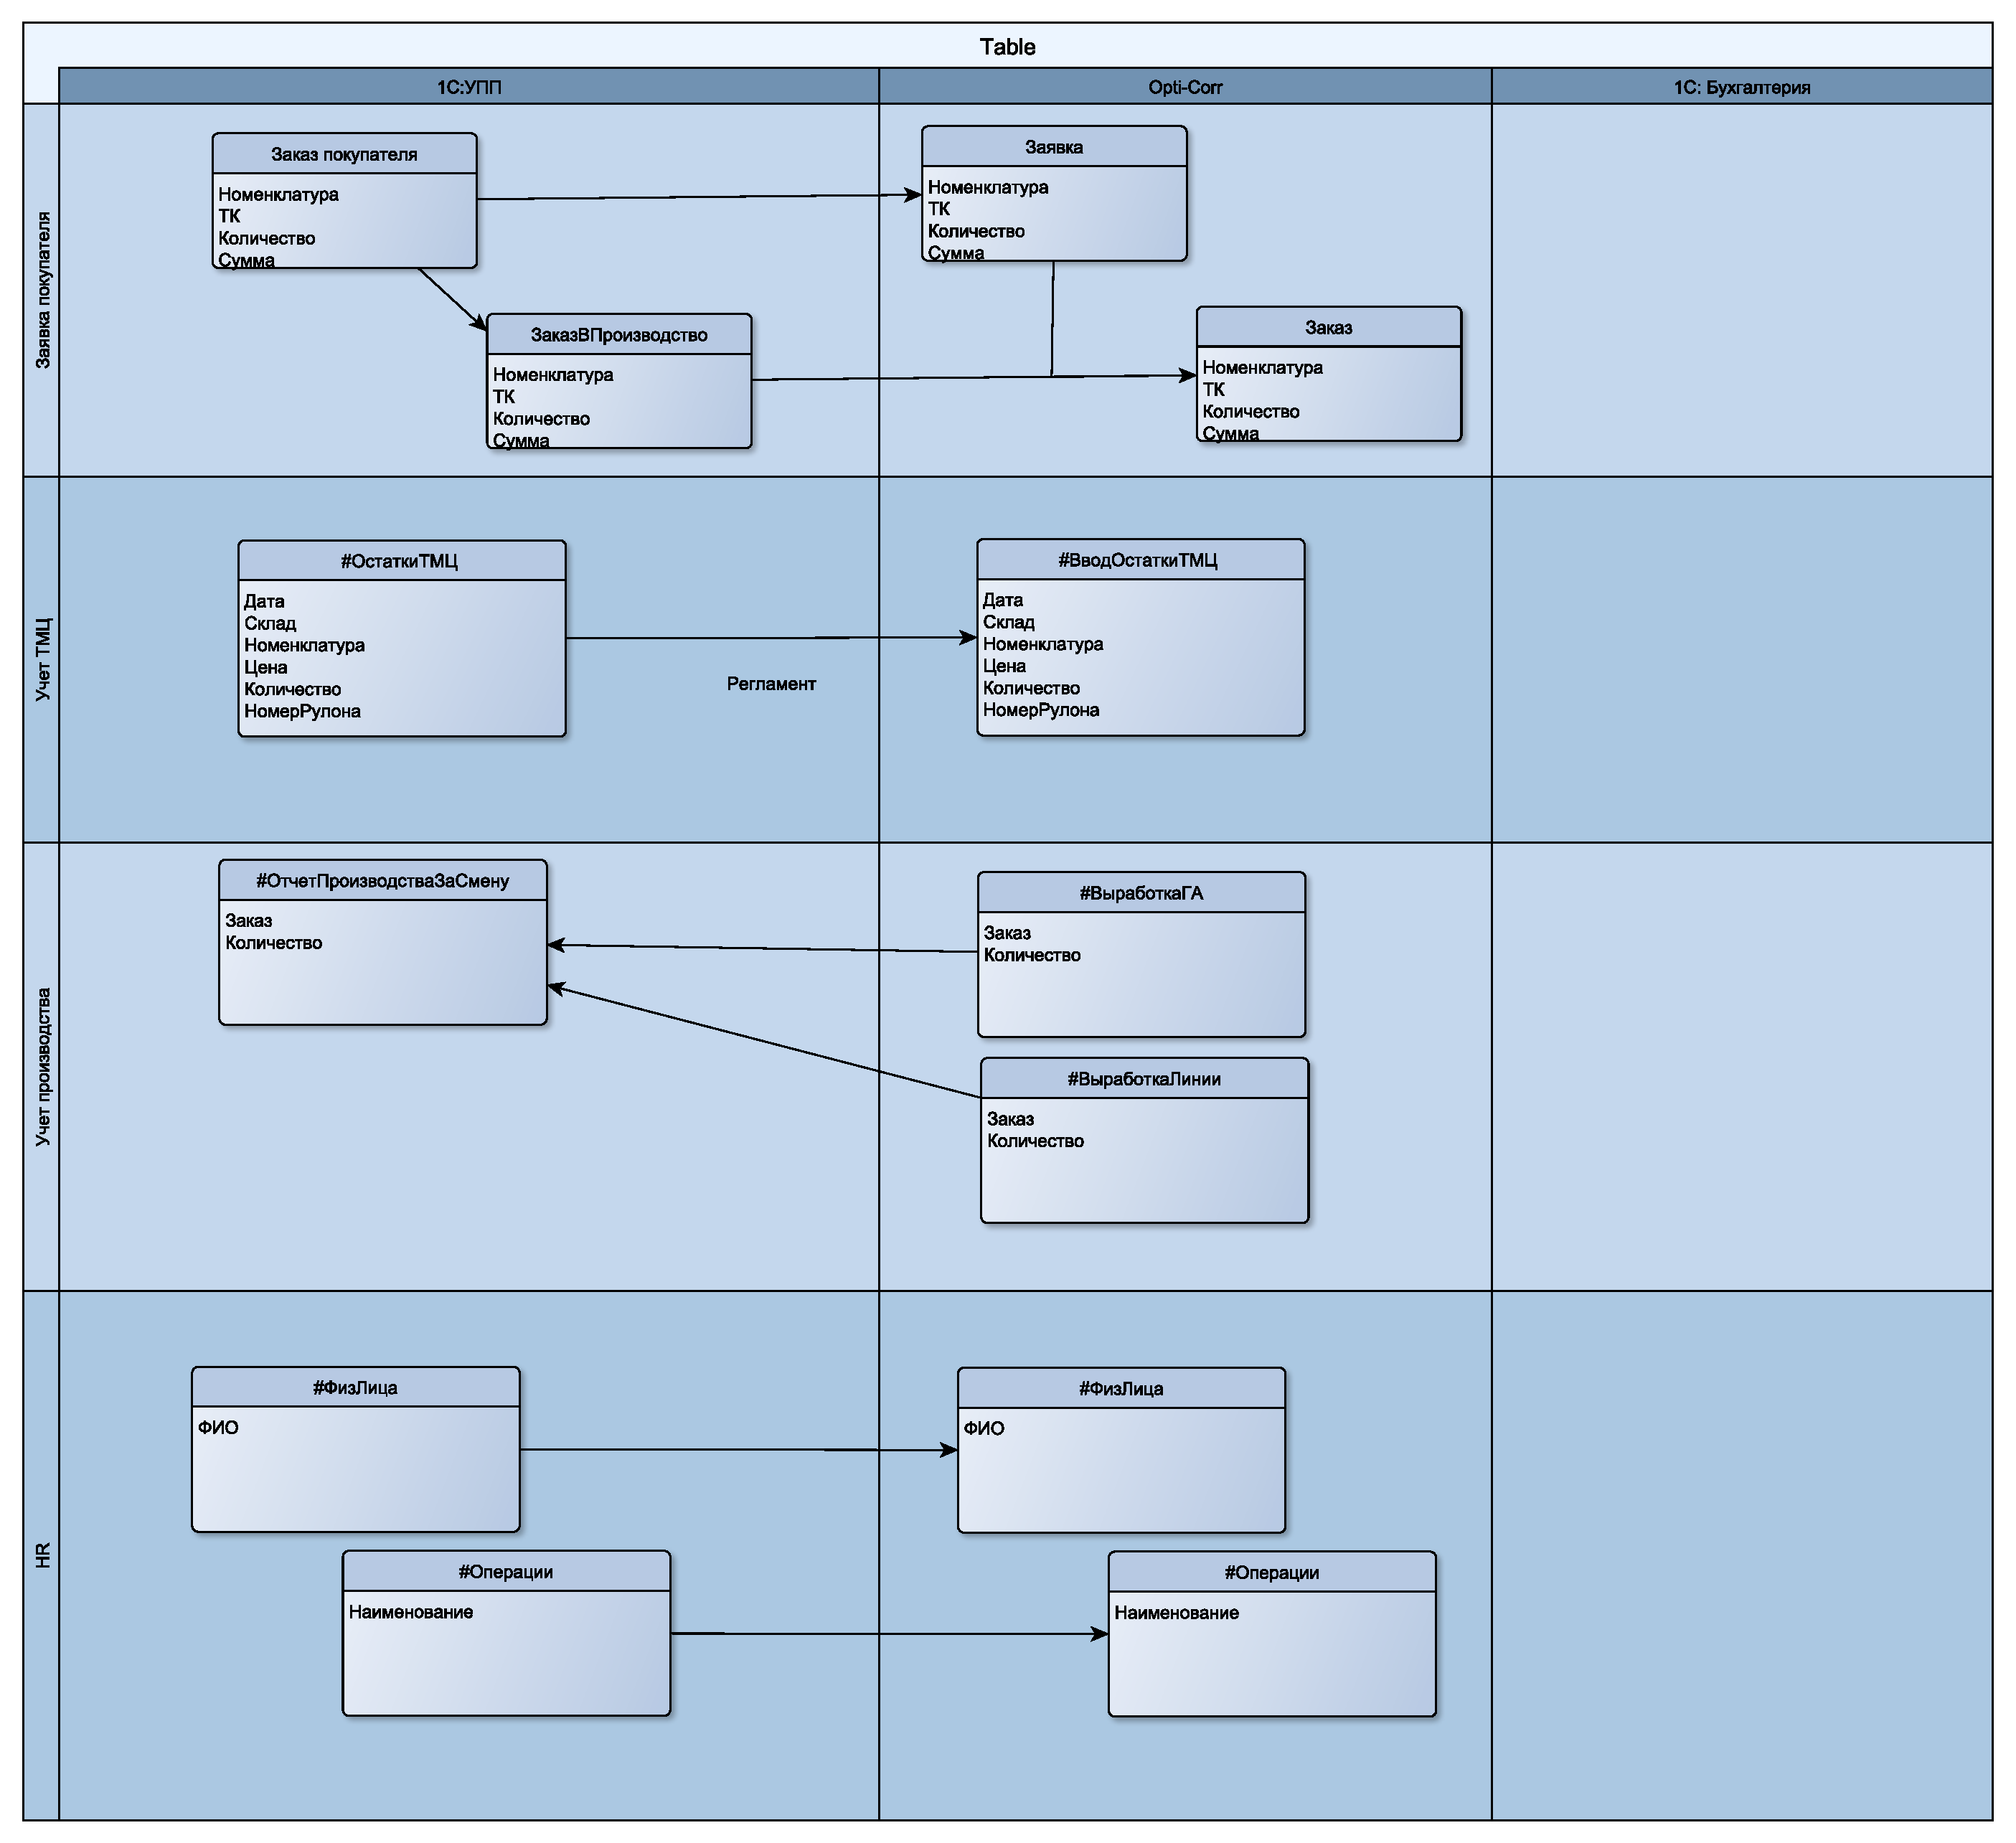
\includegraphics[height=0.8\textheight, width=1\textwidth, angle=0,  keepaspectratio]{50_Pics/DFD_2.pdf}
\end{center}
  \caption{Потоки обмена информацией между системами. Учет ТМЦ и готовой продукции}
  \label{pic:DFD_2}
\end{figure}
\FloatBarrier



% Table generated by Excel2LaTeX from sheet 'Лист1'
% \scriptsize
\begin{longtable}{|p{70mm}|p{70mm}|}
\hline
\parbox[c][19mm]{55mm}{\centering Документ 1С:УПП. Источник} & \parbox[c]{55mm}{\centering Документ Гофротары. Получатель}  \\
\hline
\parbox[c][6mm]{60mm}{Заказ покупателя} & Заявка \\
\hline
\parbox[c][6mm]{60mm}{Заказ производства} & Заказ  \\
\hline
\parbox[c][12mm]{60mm}{Остатки ТМЦ. Остатки по регистру на дату} & Ввод остатков ТМЦ  \\
\hline
\caption{Соответствие между документами для обмена}\label{tab:exchange2}
\end{longtable}  
\normalsize




% Table generated by Excel2LaTeX from sheet 'Лист1'
% \scriptsize
\begin{longtable}{|p{70mm}|p{70mm}|}
\hline
\parbox[c][19mm]{55mm}{\centering Документ Гофротары. Источник} & \parbox[c]{55mm}{\centering Соответствующий документ 1С:УПП. Получатель}  \\
\hline
\parbox[c][6mm]{60mm}{Выработка ГА} & Отчет производства за смену \\
\hline
\parbox[c][6mm]{60mm}{Выработка линии} & Отчет производства за смену \\
\hline
\caption{Соответствие между документами для обмена}\label{tab:exchange3}
\end{longtable}  
\normalsize


% \textbf{Выгрузка из OPTI-CORRUGATED в 1С: Бухгалтерия предприятия. Остатки ТМЦ}

% Источник: OPTI-CORRUGATED.

% Получатель: 1С: Бухгалтерия.

% По регламенту ежедневно в 8 утра либо принудительно по запросу необходимо из системы 1С: УПП выгружать текущие остатки по всем складам по слоям картона (Вид номенклатуры - Материалы).

% В СИСТЕМУ информация должна загружаться через вызов WEB-сервиса LoadData.

% Структура обмена


\point{Создать правило загрузки справочника ''Номенклатура'' в СИСТЕМУ}

Создать правило выгрузки из 1C: УПП в СИСТЕМУ справочника ''Номенклатура''.


Описание.

По регламенту необходимо выгружать зарегистрированные в плане обмена элементы справочника ''Номенклатура'' в части готовой продукции, номенклатуры сырья и оснастки из 1С: УПП в СИСТЕМУ.

Т.к. в 1С: УПП номенклатура ведётся в разрезе характеристик, то при передаче в СИСТЕМУ будет создано столько элементов справочника ''Номенклатура'', сколько заведено характеристик в объекте-источнике. При этом передаваемая в СИСТЕМУ номенклатура формируется по принципу ''Номенклатура + Характеристика'', и будет содержать два родительских GUID для дальнейшей синхронизации.

Синхронизация групп справочника выполняется по GUID соответствущей группы-номенклатуры.

Источник: 1С: УПП.

Объекты-источники: Номенклатура, Характеристики номенклатуры

Получатель: СИСТЕМА.

Объект получателя: Номенклатура

Параметры запроса:

% Table generated by Excel2LaTeX from sheet '20'
\scriptsize
\pc

\begin{longtable}{|p{10mm}|p{35mm}|p{40mm}|p{60mm}|}
\hline
\parbox[c][5mm]{10mm}{\centering№} & \parbox[c]{35mm}{\centeringНазвание параметра} & \parbox[c]{40mm}{\centeringТип значения} & \parbox[c]{60mm}{\centeringОписание} \\
\hline
\parbox[c][5mm]{16mm}{\p} &  GUID Номенклатуры & Уникальный идентификатор &         \\
\hline
\parbox[c][5mm]{16mm}{\p} &  GUID Характеристики & Уникальный идентификатор & Для групп не передаётся \\
\hline
%\parbox[c][5mm]{16mm}{\p} &  Код &     Строка &        Код \\
%\hline
\parbox[c][5mm]{16mm}{\p} & Наименование &     Строка & Наименование \\
\hline
\parbox[c][5mm]{16mm}{\p} & ПометкаУдаления & Булево & \\
\hline
\parbox[c][5mm]{16mm}{\p} & Полное наименование &     Строка & Полное наименование \\
\hline
\parbox[c][5mm]{16mm}{\p} & Родитель & Справочник ''Номенклатура'' & Группа \\
\hline
\parbox[c][5mm]{16mm}{\p} & GUID Тех. карты & Уникальный идентификатор & Передаётся для номенклатуры готовой продукции \\
\hline
%\parbox[c][5mm]{16mm}{\p} & Характеристика &     Строка & Характеристика номенклатуры \\
%\hline

% \parbox[c][5mm]{16mm}{\p} & Цены & Таблица Значений &            \\
% \hline
% \parbox[c][5mm]{16mm}{} & Тип цены &     Строка & Строка типа цены \\
% \hline
% \parbox[c][5mm]{16mm}{} & Дата &     Строка & Выгружается на последнюю дату изменения \\
% \hline
% \parbox[c][5mm]{16mm}{} & Значение &     Строка & Значение цены \\
% \hline
\caption{Параметры обмена справочника ''Номенклатура''}\label{ex:nomenclature}
\end{longtable}  
\normalsize

%\clearpage




\point{Создать правило загрузки справочника ''Контрагенты'' в СИСТЕМУ}

Создать правило выгрузки из 1C: УПП в СИСТЕМУ справочника ''Контрагенты''.


Описание.

По регламенту необходимо выгружать зарегистрированные в плане обмена элементы справочника ''Контрагенты'' из 1С:УПП в СИСТЕМУ.

% Синхронизация выполняется по полям ''ИНН'' и ''КПП''. В случае, если данные поля не заполнены, поиск будет осуществляться по полю ''Наименование''.
Синхронизация выполняется по GUID.

Источник: 1С:УПП.

Получатель: СИСТЕМА.

Параметры запроса:
\pc
% Table generated by Excel2LaTeX from sheet '20'
\scriptsize
\begin{longtable}{|p{10mm}|p{35mm}|p{40mm}|p{60mm}|}
\hline
\parbox[c][5mm]{10mm}{\centering№} & \parbox[c]{35mm}{\centeringНазвание параметра} & \parbox[c]{40mm}{\centeringТип значения} & \parbox[c]{60mm}{\centeringОписание} \\
\hline
\parbox[c][5mm]{16mm}{\p} &  GUID &  Уникальный идентификатор & Уникальный идентификатор \\
\hline
\parbox[c][5mm]{16mm}{\p} & Наименование &     Строка & Наименование \\
\hline
\parbox[c][5mm]{16mm}{\p} & ПометкаУдаления & Булево & \\
\hline
\parbox[c][5mm]{16mm}{\p} & Наименование полное &     Строка & Наименование полное \\
\hline
\parbox[c][5mm]{16mm}{\p} &   Родитель &  Справочник ''Контрагенты'' & Группа \\
\hline
\parbox[c][5mm]{16mm}{\p} &        ИНН &     Строка &        ИНН \\
\hline
\parbox[c][5mm]{16mm}{\p} &        КПП &     Строка &        КПП \\
\hline
\parbox[c][5mm]{16mm}{\p} & Код по ОКПО &     Строка &   Код по ОКПО \\
\hline
\parbox[c][5mm]{16mm}{\p} & Юр. / физ. лицо &  Перечисление & Юр. / физ. лицо  \\
\hline
\parbox[c][5mm]{16mm}{\p} & Основной договор & Справочник ''Договоры контрагентов'' & Основной договор контрагента \\
\hline
% \parbox[c][5mm]{16mm}{6} & Номер счета &     Строка & Номер счета \\
% \hline
% \parbox[c][5mm]{16mm}{7} &    Код БИК &     Строка &    Код БИК \\
% \hline
\caption{Параметры обмена справочника ''Контрагенты''}\label{ex:customer}
\end{longtable}  
\normalsize




\point{Создать правило загрузки справочника ''Договоры контрагентов'' в СИСТЕМУ}

Создать правило выгрузки из 1C: УПП в СИСТЕМУ справочника ''Договоры контрагентов''.


Описание.

По регламенту необходимо выгружать зарегистрированные в плане обмена элементы справочника ''Договоры контрагентов'' из 1C: УПП в СИСТЕМУ.

%Синхронизация выполняется по полям ''Номер договора'', ''Дата договора'' и ''Владелец'' (Контрагент).
Синхронизация выполняется по GUID.

Источник: 1С: УПП.

Получатель: СИСТЕМА.

Параметры запроса:
\pc
% Table generated by Excel2LaTeX from sheet '20'
\scriptsize
\begin{longtable}{|p{10mm}|p{35mm}|p{40mm}|p{60mm}|}
\hline
\parbox[c][5mm]{10mm}{\centering№} & \parbox[c]{35mm}{\centeringНазвание параметра} & \parbox[c]{40mm}{\centeringТип значения} & \parbox[c]{60mm}{\centeringОписание} \\
\hline
\parbox[c][5mm]{16mm}{\p} & GUID & Уникальный идентификатор & Уникальный идентификатор \\
\hline
\parbox[c][5mm]{16mm}{\p} & Наименование &  Строка & Наименование \\
\hline
\parbox[c][5mm]{16mm}{\p} & ПометкаУдаления & Булево & \\
\hline
\parbox[c][5mm]{16mm}{\p} & Владелец & Справочник ''Контрагенты'' & Контрагент \\
\hline
\parbox[c][5mm]{16mm}{\p} & Номер & Строка & Номер договора \\
\hline
\parbox[c][5mm]{16mm}{\p} & Дата & Строка & Дата договора \\
\hline
\parbox[c][5mm]{16mm}{\p} & Вид договора & Перечисление & Вид договора \\
\hline
\parbox[c][5mm]{16mm}{\p} & Организация &  Справочник ''Организации'' & Организация \\
\hline
\parbox[c][5mm]{16mm}{\p} & Тип цен &  Справочник ''Типы цен'' & Тип цен \\
\hline
\parbox[c][5mm]{16mm}{\p} & Валюта &  Справочник ''Валюты'' & Валюта взаиморасчётов \\
\hline
\parbox[c][5mm]{16mm}{\p} & СуммаКредита & Число & Допустимая сумма задолженности \\
\hline
\parbox[c][5mm]{16mm}{\p} & СрокКредита & Число & Допустимое число дней задолженности \\
\hline
\parbox[c][5mm]{16mm}{\p} & КонтролироватьКредит & Булево & Контролировать число дней задолженности \\
\hline
% \parbox[c][5mm]{16mm}{3} & Валюта взаиморасчетов &     Справочник ''Валюты'' & Валюта договора \\
% \hline
% \parbox[c][5mm]{16mm}{3} & Срок кредита & Число & Допустимое число дней задолженности \\
% \hline
% \parbox[c][5mm]{16mm}{3} & Сумма кредита & Число & Допустимая сумма задолженности \\
%\hline

\caption{Параметры обмена справочника ''Договоры контрагентов''}\label{ex:contract}
\end{longtable}  
\normalsize



\point{Создать правило загрузки справочника ''Склады'' в СИСТЕМУ}

Создать правило выгрузки из 1C: УПП в СИСТЕМУ справочника ''Склады''.


Описание.

По регламенту необходимо выгружать зарегистрированные в плане обмена элементы справочника ''Склады'' из  1C: УПП в СИСТЕМУ.

%Синхронизация выполняется по полям ''Код''.
Синхронизация выполняется по GUID.

Источник: 1С: УПП.

Объект-источник: Справочник ''Склады'' 

Получатель: СИСТЕМА.

Объект-получатель: Справочник ''Структурные единицы''

Параметры запроса:
\pc
% Table generated by Excel2LaTeX from sheet '20'
\scriptsize
\begin{longtable}{|p{10mm}|p{35mm}|p{40mm}|p{60mm}|}
\hline
\parbox[c][5mm]{10mm}{\centering№} & \parbox[c]{35mm}{\centeringНазвание параметра} & \parbox[c]{40mm}{\centeringТип значения} & \parbox[c]{60mm}{\centeringОписание} \\
\hline
\parbox[c][5mm]{16mm}{\p} & GUID & Уникальный идентификатор & Уникальный идентификатор \\
\hline
\parbox[c][5mm]{16mm}{\p} & Наименование &     Строка & Наименование \\
\hline
\parbox[c][5mm]{16mm}{\p} & ПометкаУдаления & Булево & \\
\hline
% \hline
% \parbox[c][5mm]{16mm}{3} & Валюта взаиморасчетов &     Справочник ''Валюты'' & Валюта договора \\
% \hline
% \parbox[c][5mm]{16mm}{3} & Срок кредита & Число & Допустимое число дней задолженности \\
% \hline
% \parbox[c][5mm]{16mm}{3} & Сумма кредита & Число & Допустимая сумма задолженности \\
% \hline

\caption{Параметры обмена справочника ''Склады''}\label{ex:contract}
\end{longtable}  
\normalsize


\point{Создать правило загрузки справочника ''Физические лица'' в СИСТЕМУ}

Создать правило выгрузки из СИСТЕМЫ из  1C: УПП в СИСТЕМУ справочника ''Физические лица''.

% СправочникСсылка.ФизическиеЛица
Описание.

По регламенту необходимо выгружать зарегистрированные в плане обмена элементы справочника ''Физические лица'' из 1C: УПП в СИСТЕМУ.

%Синхронизация выполняется по полям ''Код''.
Синхронизация выполняется по GUID.

Источник: 1С: УПП.

Объект-источник: Справочник ''Физические лица'' 

Получатель: СИСТЕМА.

Объект-получатель: Справочник ''Физические лица''

Параметры запроса:
\pc
% Table generated by Excel2LaTeX from sheet '20'
\scriptsize
\begin{longtable}{|p{10mm}|p{35mm}|p{40mm}|p{60mm}|}
\hline
\parbox[c][5mm]{10mm}{\centering№} & \parbox[c]{35mm}{\centeringНазвание параметра} & \parbox[c]{40mm}{\centeringТип значения} & \parbox[c]{60mm}{\centeringОписание} \\
\hline
\parbox[c][5mm]{16mm}{\p} & GUID & Уникальный идентификатор & Уникальный идентификатор \\
\hline
\parbox[c][5mm]{16mm}{\p} & Наименование &     Строка & Наименование \\
\hline
\parbox[c][5mm]{16mm}{\p} & ПометкаУдаления & Булево & \\
\hline
\parbox[c][5mm]{16mm}{\p} & Родитель & Справочник ''Физические лица'' & Группа \\
\hline
\parbox[c][5mm]{16mm}{\p} & Должность  & Строка & Наименование должности \\
\hline
\caption{Параметры обмена справочник ''Физические лица''}\label{ex:workers}
\end{longtable}  
\normalsize



\point{Создать правило загрузки справочника ''Подразделения'' в СИСТЕМУ}

Создать правило выгрузки из  1C: УПП в СИСТЕМУ справочника ''Подразделения''.

% СправочникСсылка.ФизическиеЛица
Описание.

По регламенту необходимо выгружать зарегистрированные в плане обмена элементы справочника ''Подразделения'' из 1C: УПП в СИСТЕМУ.

%Синхронизация выполняется по полям ''Код''.
Синхронизация выполняется по GUID.

Источник: 1С: УПП.

Объект-источник: Справочник ''Подразделения'' 

Получатель: СИСТЕМА.

Объект-получатель: Справочник ''Структурные единицы''

Параметры запроса:
\pc
% Table generated by Excel2LaTeX from sheet '20'
\scriptsize
\begin{longtable}{|p{10mm}|p{35mm}|p{40mm}|p{60mm}|}
\hline
\parbox[c][5mm]{10mm}{\centering№} & \parbox[c]{35mm}{\centeringНазвание параметра} & \parbox[c]{40mm}{\centeringТип значения} & \parbox[c]{60mm}{\centeringОписание} \\
\hline
\parbox[c][5mm]{16mm}{\p} & GUID & Уникальный идентификатор & Уникальный идентификатор \\
\hline
\parbox[c][5mm]{16mm}{\p} & Наименование &     Строка & Наименование \\
\hline
\parbox[c][5mm]{16mm}{\p} & ПометкаУдаления & Булево & \\
\hline
% \hline
%\parbox[c][5mm]{16mm}{3} & Родитель &     Строка & Наименование родительской группы \\
%\hline

\caption{Параметры обмена справочника ''Подразделения''}\label{ex:workers}
\end{longtable}  
\normalsize




\point{Создать WEB-сервис Загрузить технологическую карту}
\label{ex:LoadDesign}

Создать WEB-сервис по выгрузке из системы 1C: УПП элемента справочника ''Технологические карты''.
Сервис должен использоваться для первоначальной загрузки данных по техкартам. 
В дальнейшей работе для загрузки техкарт необходимо использовать сервис загрузки в документы ''Заявка-Спецификация''.

Имя сервиса: LoadDesign.

Описание.

По событию команде \#СоздатьТехнологическуюКарту в системе 1С: УПП должен вызываться WEB-сервис создания записи справочника Технологическая карта в СИСТЕМЕ.

Сервис должен создать новый элемент справочника Технологические карты, заполнить свойства элемента параметрами, переданными на вход сервиса.

Параметры запроса:
\pc
% Table generated by Excel2LaTeX from sheet '1'
\scriptsize
\begin{longtable}{|p{10mm}|p{35mm}|p{40mm}|p{60mm}|}
\hline
\parbox[c][5mm]{10mm}{\centering№} & \parbox[c]{35mm}{\centeringНазвание параметра} & \parbox[c]{40mm}{\centeringТип значения} & \parbox[c]{60mm}{\centeringОписание} \\
\hline
\parbox[c][5mm]{9mm}{\p} & Наименование гофропродукции &     Строка & Наименование изделия \\
\hline
\parbox[c][5mm]{9mm}{\p} &  Менеджер & Уникальный идентификатор & GUID менеджера \\
\hline
\parbox[c][5mm]{9mm}{\p} &  ВидГофропродукции & Строка &  {Наименование типа изделия. Справочник. Синхронизация по коду}. \\
\hline
\parbox[c][5mm]{9mm}{\p} &  ЕдиницаИзмерения & Строка &  {Единица измерения. Справочник. Синхронизация по коду} \\
\hline
\parbox[c][5mm]{9mm}{\p} &  ГОСТ\_ТУ & Строка &  {Наименование ГОСТа} \\
\hline
\parbox[c][5mm]{9mm}{\p} &  ДлинаЯщика & Число &  {Длина ящика} \\
\hline
\parbox[c][5mm]{9mm}{\p} &  ШиринаЯщика & Число &  {Ширина ящика} \\
\hline
\parbox[c][5mm]{9mm}{\p} &  ВысотаЯщика & Число &  {Высота ящика} \\
\hline
\parbox[c][5mm]{9mm}{\p} &  ЦветМарки & Строка &  {Цвет картона. Справочник. Синхронизация по коду.} \\
\hline
\parbox[c][5mm]{9mm}{\p} &  КоличествоИзделийПакет & Число &  {Количество изделий в пачке} \\
\hline
\parbox[c][5mm]{9mm}{\p} &  Поддон & Строка &  {Поддон. Справочник. Синхронизация по коду.} \\
\hline
\parbox[c][5mm]{9mm}{\p} &  СтрейчПпленка & Булево &  {Упаковка в пленку} \\
\hline
\parbox[c][5mm]{9mm}{\p} &  Крышка & Булево &  {Необходимость в крышке} \\
\hline
\parbox[c][5mm]{9mm}{\p} &  Уголки & Булево &  {Необходимость в уголках} \\
\hline
\parbox[c][5mm]{9mm}{\p} &  МаркаКартона & Строка &  {Марка картона. Справочник. Синхронизация по наименованию.} \\
\hline
\parbox[c][5mm]{9mm}{\p} &  ТипыРилевок & Строка &  {Тип рилевок. Справочник. Синхронизация по коду.} \\
\hline
\parbox[c][5mm]{9mm}{\p} &  Профиль & Строка &  {Профиль картона. Справочник. Синхронизация по наименованию.} \\
\hline
\parbox[c][5mm]{9mm}{\p} &  Количествовпачке & Число &  {Количество в пачке} \\
\hline
\parbox[c][5mm]{9mm}{\p} &  КоличествоПачекВРяд & Число &  {Количество пачек в ряд} \\
\hline
\parbox[c][5mm]{9mm}{\p} &  КоличествоРядов & Число &  {Количество рядов} \\
\hline
\parbox[c][5mm]{9mm}{\p} &  ТипУпаковки & Строка &  {Тип упаковки. Справочник. Синхронизация по коду.} \\
\hline
\parbox[c][5mm]{9mm}{\p} &  ТипПоддона & Строка &  {Тип поддона. Справочник. Синхронизация по коду.} \\
\hline
\parbox[c][5mm]{9mm}{\p} &  Укладка & Строка &  {Шаблон схемы упаковки. Справочник. Синхронизация по коду.} \\
\hline
\parbox[c][5mm]{9mm}{\p} &  Файлы & \parbox{52mm}{Base64} &  {Список файлов в формате Base54} \\
\hline
\parbox[c][5mm]{9mm}{\p} &  ДлинаЗаготовки & Число &  {Длина заготовки} \\
\hline
\parbox[c][5mm]{9mm}{\p} &  ШиринаЗаготовки & Число &  {Ширина заготовки} \\
\hline
\parbox[c][5mm]{9mm}{\p} &  ПлощадьЗаготовки & Число &  {Площадь заготовки} \\
\hline
\parbox[c][5mm]{9mm}{\p} &  Позиционность & Число &  {Кратность} \\
\hline
\parbox[c][5mm]{9mm}{\p} &  GUID Номенклатуры & Уникальный идентификатор  &  {GUID Номенклатуры} \\
\hline
\parbox[c][5mm]{9mm}{\p} &  GUID Характеристики & Уникальный идентификатор &  {GUID Характеристики} \\
\hline
\parbox[c][5mm]{9mm}{\p} &  Заметки & Строка &  {Дополнительные  требования} \\
\hline
\caption{Параметры запроса LoadSpecification}\label{ex:in_LoadDesign}
\end{longtable}  
\normalsize



Параметры ответа
\pc
% Table generated by Excel2LaTeX from sheet '1'
\scriptsize
\begin{longtable}{|p{10mm}|p{40mm}|p{20mm}|p{75mm}|}
\hline
\parbox[c][5mm]{10mm}{\centering№} & \parbox[c]{40mm}{\centeringНазвание параметра} & \parbox[c]{20mm}{\centeringТип значения} & \parbox[c]{75mm}{\centeringОписание} \\
\hline
\parbox[c][5mm]{15mm}{\p} & \parbox{70mm}{GUID Техкарты} & \parbox{54mm}{Строка} & \parbox{49mm}{GUID созданного элемента} \\
\hline
\parbox[c][5mm]{15mm}{\p} & \parbox{70mm}{GUID Заявки-Спецификации} & \parbox{54mm}{Строка} & \parbox{49mm}{GUID созданного документа} \\
\hline
\parbox[c][5mm]{15mm}{\p} & \parbox{70mm}{Текст ошибки} & \parbox{54mm}{Строка} & \parbox{49mm}{Текст ошибки при создании} \\
\hline
\caption{Параметры ответа LoadSpecification}\label{ex:out_LoadDesign}
\end{longtable}  
\normalsize




\point{Создать WEB-сервис Загрузить заявку-спецификацию}
\label{ex:LoadSpecification}

Создать WEB-сервис по выгрузке из системы 1C: УПП элемента справочника ''Технологические карты''.

Имя сервиса: LoadSpecification.

Описание.

По событию команде \#СоздатьЗаявкуСпецификацию в системе 1С: УПП должен вызываться WEB-сервис создания нового документа ''Заявка-Спецификация'' в СИСТЕМЕ.

Сервис должен создать новый документ ''Заявка-Спецификация'' в СИСТЕМЕ, заполнить свойства элемента параметрами, переданными на вход сервиса.

При создании документа необходимо автоматически создавать новый элемент справочника ''Технологическая карта''. Ссылка на созданный элемент сохраняется в документе ''Заявка-Спецификация'' и должна быть передана в качестве ответ на работу сервиса.

Параметры запроса:
\pc
% Table generated by Excel2LaTeX from sheet '1'
\scriptsize
\begin{longtable}{|p{10mm}|p{35mm}|p{40mm}|p{60mm}|}
\hline
\parbox[c][5mm]{10mm}{\centering№} & \parbox[c]{35mm}{\centeringНазвание параметра} & \parbox[c]{40mm}{\centeringТип значения} & \parbox[c]{60mm}{\centeringОписание} \\
\hline
\parbox[c][5mm]{9mm}{\p} & Наименование гофропродукции &     Строка & Наименование изделия \\
\hline
\parbox[c][5mm]{9mm}{\p} &  Менеджер & Уникальный идентификатор & GUID менеджера \\
\hline
\parbox[c][5mm]{9mm}{\p} &  ВидГофропродукции & Строка &  {Наименование типа изделия. Справочник. Синхронизация по коду}. \\
\hline
\parbox[c][5mm]{9mm}{\p} &  ЕдиницаИзмерения & Строка &  {Единица измерения. Справочник. Синхронизация по коду} \\
\hline
\parbox[c][5mm]{9mm}{\p} &  ГОСТ\_ТУ & Строка &  {Наименование ГОСТа} \\
\hline
\parbox[c][5mm]{9mm}{\p} &  ДлинаЯщика & Число &  {Длина ящика} \\
\hline
\parbox[c][5mm]{9mm}{\p} &  ШиринаЯщика & Число &  {Ширина ящика} \\
\hline
\parbox[c][5mm]{9mm}{\p} &  ВысотаЯщика & Число &  {Высота ящика} \\
\hline
\parbox[c][5mm]{9mm}{\p} &  ЦветМарки & Строка &  {Цвет картона. Справочник. Синхронизация по коду.} \\
\hline
\parbox[c][5mm]{9mm}{\p} &  КоличествоИзделийПакет & Число &  {Количество изделий в пачке} \\
\hline
\parbox[c][5mm]{9mm}{\p} &  Поддон & Строка &  {Поддон. Справочник. Синхронизация по коду.} \\
\hline
\parbox[c][5mm]{9mm}{\p} &  СтрейчПпленка & Булево &  {Упаковка в пленку} \\
\hline
\parbox[c][5mm]{9mm}{\p} &  Крышка & Булево &  {Необходимость в крышке} \\
\hline
\parbox[c][5mm]{9mm}{\p} &  Уголки & Булево &  {Необходимость в уголках} \\
\hline
\parbox[c][5mm]{9mm}{\p} &  МаркаКартона & Строка &  {Марка картона. Справочник. Синхронизация по наименованию.} \\
\hline
\parbox[c][5mm]{9mm}{\p} &  ТипыРилевок & Строка &  {Тип рилевок. Справочник. Синхронизация по коду.} \\
\hline
\parbox[c][5mm]{9mm}{\p} &  Профиль & Строка &  {Профиль картона. Справочник. Синхронизация по наименованию.} \\
\hline
\parbox[c][5mm]{9mm}{\p} &  Количествовпачке & Число &  {Количество в пачке} \\
\hline
\parbox[c][5mm]{9mm}{\p} &  КоличествоПачекВРяд & Число &  {Количество пачек в ряд} \\
\hline
\parbox[c][5mm]{9mm}{\p} &  КоличествоРядов & Число &  {Количество рядов} \\
\hline
\parbox[c][5mm]{9mm}{\p} &  ТипУпаковки & Строка &  {Тип упаковки. Справочник. Синхронизация по коду.} \\
\hline
\parbox[c][5mm]{9mm}{\p} &  ТипПоддона & Строка &  {Тип поддона. Справочник. Синхронизация по коду.} \\
\hline
\parbox[c][5mm]{9mm}{\p} &  Укладка & Строка &  {Шаблон схемы упаковки. Справочник. Синхронизация по коду.} \\
\hline
\parbox[c][5mm]{9mm}{\p} &  Файлы & \parbox{52mm}{Base64} &  {Список файлов в формате Base54} \\
\hline
\parbox[c][5mm]{9mm}{\p} &  ДлинаЗаготовки & Число &  {Длина заготовки} \\
\hline
\parbox[c][5mm]{9mm}{\p} &  ШиринаЗаготовки & Число &  {Ширина заготовки} \\
\hline
\parbox[c][5mm]{9mm}{\p} &  ПлощадьЗаготовки & Число &  {Площадь заготовки} \\
\hline
\parbox[c][5mm]{9mm}{\p} &  Позиционность & Число &  {Кратность} \\
\hline
\parbox[c][5mm]{9mm}{\p} &  GUID Номенклатуры & Уникальный идентификатор  &  {GUID Номенклатуры} \\
\hline
\parbox[c][5mm]{9mm}{\p} &  GUID Характеристики & Уникальный идентификатор &  {GUID Характеристики} \\
\hline
\parbox[c][5mm]{9mm}{\p} &  Заметки & Строка &  {Дополнительные  требования} \\
\hline
\caption{Параметры запроса LoadSpecification}\label{ex:in_LoadSpecification}
\end{longtable}  
\normalsize



Параметры ответа
\pc
% Table generated by Excel2LaTeX from sheet '1'
\scriptsize
\begin{longtable}{|p{5mm}|p{40mm}|p{40mm}|p{60mm}|}
\hline
\parbox[c][5mm]{5mm}{\centering№} & \parbox[c]{40mm}{\centeringНазвание параметра} & \parbox[c]{40mm}{\centeringТип значения} & \parbox[c]{60mm}{\centeringОписание} \\
\hline
\parbox[c][5mm]{15mm}{\p} & \parbox{70mm}{GUID Техкарты} & \parbox{54mm}{Уникальный идентификатор} & \parbox{49mm}{GUID созданного элемента} \\
\hline
\parbox[c][5mm]{15mm}{\p} & \parbox{70mm}{GUID Заявки-Спецификации} & \parbox{54mm}{Уникальный идентификатор} & \parbox{49mm}{GUID созданного документа} \\
\hline
\parbox[c][5mm]{15mm}{\p} & \parbox{70mm}{Текст ошибки} & \parbox{54mm}{Строка} & \parbox{49mm}{Текст ошибки при создании} \\
\hline
\caption{Параметры ответа LoadSpecification}\label{ex:outLout_Specification}
\end{longtable}  
\normalsize




\point{Создать WEB-сервис Загрузить заказ покупателя}
\label{exchange:LoadSalesOrder}

 Создать WEB-сервис по выгрузке заказа покупателя из системы 1С: УПП.
 Сервис должен вызываться из системы 1С: УПП из документа ''Заказ покупателя''.
 
 % Перед загрузкой документа необходимо вызвать сервис расчета даты заказа (Объемно-календарное планирование) для проверки рассчитанной даты производства.
 % Если рассчитанная дата не совпадает с параметром Желаемая дата отгрузки, загрузка должна выполняться, сервис должен вернуть сообщение об ошибке с указанием причины, по которой производство невозможно. 
 
 Сервис должен загружать документ ''Заказ покупателя'' системы 1С: УПП в документ ''Заявка'' СИСТЕМЫ.
 
 При этом по каждой строке Заказа покупателя необходимо создать в СИСТЕМЕ документ ''Заказ'' по загруженному документу ''Заказ''.
 
 Получатели: СИСТЕМА.

 Имя сервиса: LoadSalesOrder.

% Описание.
 
% Сервис должен по запросу формировать список оборудования и текущего состояния по простоям по регистру ''Журнал работы оборудования''.

% При типе запроса 0 возвращать срез последнего состояния по каждому оборудованию.

% При типе запроса 1 возвращать выборку всех событий по каждому оборудованию за период.


Параметры запроса:
\pc
% Table generated by Excel2LaTeX from sheet '7'
\scriptsize
\begin{longtable}{|p{10mm}|p{35mm}|p{40mm}|p{60mm}|}
\hline
\parbox[c][5mm]{10mm}{\centering№} & \parbox[c]{35mm}{\centeringНазвание параметра} & \parbox[c]{40mm}{\centeringТип значения} & \parbox[c]{60mm}{\centeringОписание} \\
\hline
\parbox[c][5mm]{16mm}{\p} & GUID & Уникальный идентификатор & Уникальный идентификатор \\
\hline
\parbox[c][5mm]{11mm}{\p} & Номер документа & Строка & Номер документа \\
\hline
\parbox[c][5mm]{11mm}{\p} & Дата документа & Дата & Дата документа \\
\hline
\parbox[c][5mm]{11mm}{\p} & Контрагент & Уникальный идентификатор & GUID контрагента \\
\hline
\parbox[c][5mm]{11mm}{\p} & Договор &  Уникальный идентификатор  & GUID договора \\
\hline
\parbox[c][5mm]{11mm}{\p} & Организация & Уникальный идентификатор & GUID организации \\
\hline
\parbox[c][5mm]{11mm}{\p} & Комментарий & Строка & Комментарий \\
\hline
\parbox[c][5mm]{11mm}{\p} & Номенклатура & Таблица значений & \\
\hline
\parbox[c][5mm]{11mm}{} & GUID Техкарты & Уникальный идентификатор   & GUID технологической карты \\
%\hline
\parbox[c][5mm]{11mm}{} & Количество & Число & Количество продукции \\
%\hline
\parbox[c][5mm]{11mm}{} & Желаемая дата отгрузки & Дата & Желаемая дата отгрузки \\
%\hline
\parbox[c][5mm]{11mm}{} & Цена & Число & Цена \\
%\hline
\parbox[c][5mm]{11mm}{} &  Ставка НДС & Число & Ставка НДС \\
%\hline
\parbox[c][5mm]{11mm}{} & Сумма НДС & Число & Сумма НДС \\
%\hline
\parbox[c][5mm]{11mm}{} & Всего & Число & Всего \\
\hline
\caption{Параметры запроса LoadSalesOrder}\label{ex:in_LoadSalesOrder}
\end{longtable}  
\normalsize



 
Параметры ответа:
\pc
% Table generated by Excel2LaTeX from sheet '7'
\scriptsize
\begin{longtable}{|p{10mm}|p{40mm}|p{20mm}|p{75mm}|}
\hline
\parbox[c][5mm]{10mm}{\centering№} & \parbox[c]{40mm}{\centeringНазвание параметра} & \parbox[c]{20mm}{\centeringТип значения} & \parbox[c]{75mm}{\centeringОписание} \\
\hline
\parbox[c][5mm]{15mm}{\p} & \parbox[c]{30mm}{\raggedrightРезультат} & \parbox[c]{50mm}{Строка}  & \parbox[c]{75mm}{Результат выполнения} \\
\hline
\caption{Параметры ответа LoadSalesOrder}\label{ex:out_LoadSalesOrder}
\end{longtable}  
\normalsize





\point{Создать WEB-сервис Загрузить заказ на производство}
\label{exchange:LoadWorkOrder}

 Создать WEB-сервис по выгрузке заказа на производство из системы 1С: УПП.
 Сервис должен вызываться из системы 1С: УПП из документа ''Заказ на производство''.
 
 % Перед загрузкой документа необходимо вызвать сервис расчета даты заказа (Объемно-календарное планирование) для проверки рассчитанной даты производства.
 % Если рассчитанная дата не совпадает с параметром Желаемая дата отгрузки, загрузка должна выполняться, сервис должен вернуть сообщение об ошибке с указанием причины, по которой производство невозможно. 
 
 Сервис должен загружать документ ''Заказ на производство'' системы 1С: УПП в документ ''Заказ'' СИСТЕМЫ.

 В документе ''Заказ на производство'' в системе 1С:УПП должна быть только одна строка в табличной части документа ''Продукция''.
 % При этом по каждой строке Заказа покупателя необходимо создать в СИСТЕМЕ документ ''Заказ'' по загруженному документу ''Заказ''.
 
Источник: 1С: УПП.

Объект-источник: Документ ''Заказ на производство'' 

Получатель: СИСТЕМА.

Объект-получатель: Документ ''Заказ''

 Имя сервиса: LoadWorkOrder.

% Описание.
 
% Сервис должен по запросу формировать список оборудования и текущего состояния по простоям по регистру ''Журнал работы оборудования''.

% При типе запроса 0 возвращать срез последнего состояния по каждому оборудованию.

% При типе запроса 1 возвращать выборку всех событий по каждому оборудованию за период.


Параметры запроса:
\pc
% Table generated by Excel2LaTeX from sheet '7'
\scriptsize
\begin{longtable}{|p{10mm}|p{35mm}|p{40mm}|p{60mm}|}
\hline
\parbox[c][5mm]{10mm}{\centering№} & \parbox[c]{35mm}{\centeringНазвание параметра} & \parbox[c]{40mm}{\centeringТип значения} & \parbox[c]{60mm}{\centeringОписание} \\
\hline
\parbox[c][5mm]{16mm}{\p} & GUID & Уникальный идентификатор & Уникальный идентификатор \\
\hline
\parbox[c][5mm]{11mm}{\p} & Номер документа & Строка & Номер документа \\
\hline
\parbox[c][5mm]{11mm}{\p} & Дата документа & Дата & Дата документа \\
\hline
\parbox[c][5mm]{11mm}{\p} & Контрагент & Уникальный идентификатор & GUID контрагента \\
\hline
\parbox[c][5mm]{11mm}{\p} & Договор & Уникальный идентификатор & GUID договора \\
\hline
\parbox[c][5mm]{11mm}{\p} & Организация & Уникальный идентификатор & GUID организации \\
\hline
\parbox[c][5mm]{11mm}{\p} & Комментарий & Строка & Комментарий \\
\hline
\parbox[c][5mm]{11mm}{\p} & GUID заказа покупателя & Уникальный идентификатор & GUID заказа покупателя \\
\hline
\parbox[c][5mm]{11mm}{\p} & GUID Номенклатуры & Уникальный идентификатор & GUID номенклатуры \\
\hline
\parbox[c][5mm]{11mm}{\p} & GUID Характеристики & Уникальный идентификатор & GUID характеристики номенклатуры \\
\hline
\parbox[c][5mm]{11mm}{\p} & GUID Техкарты & Уникальный идентификатор & GUID технологической карты \\
\hline
\parbox[c][5mm]{11mm}{\p} & Количество & Число & Количество продукции \\
\hline
\parbox[c][5mm]{11mm}{\p} & Желаемая дата отгрузки & Дата & Желаемая дата отгрузки \\
\hline
\caption{Параметры запроса LoadWorkOrder}\label{ex:in_LoadWorkOrder}
\end{longtable}  
\normalsize



 
Параметры ответа:
\pc
% Table generated by Excel2LaTeX from sheet '7'
\scriptsize
\begin{longtable}{|p{10mm}|p{40mm}|p{20mm}|p{75mm}|}
\hline
\parbox[c][5mm]{10mm}{\centering№} & \parbox[c]{40mm}{\centeringНазвание параметра} & \parbox[c]{20mm}{\centeringТип значения} & \parbox[c]{75mm}{\centeringОписание} \\
\hline
\parbox[c][5mm]{15mm}{\p} & \parbox[c]{30mm}{\raggedrightРезультат} & \parbox[c]{50mm}{Строка}  & \parbox[c]{75mm}{Результат выполнения} \\
\hline
\caption{Параметры ответа LoadWorkOrder}\label{ex:out_LoadWorkOrder}
\end{longtable}  
\normalsize







% Обмен из СИСТЕМЫ во внешнюю

\point{Создать WEB-сервис Получить статус техкарты}
\label{exchange:GetDesignStatus}

 Создать WEB-сервис по получению информации по статусу технологической карты при заведении заказа покупателя в системе 1С: УПП.
 Сервис должен вызываться из системы 1С: УПП и возвращать текущее состояние технологической карты для контроля ввода номенклатуры продукции в документе ''Заказ покупателя''.

 Получатели: система 1С: УПП.

 Имя сервиса: GetDesignStatus.

% Описание.
 
% Сервис должен по запросу формировать список оборудования и текущего состояния по простоям по регистру ''Журнал работы оборудования''.

% При типе запроса 0 возвращать срез последнего состояния по каждому оборудованию.

% При типе запроса 1 возвращать выборку всех событий по каждому оборудованию за период.


Параметры запроса:
\pc
% Table generated by Excel2LaTeX from sheet '7'
\scriptsize
\begin{longtable}{|p{10mm}|p{35mm}|p{40mm}|p{60mm}|}
\hline
\parbox[c][5mm]{10mm}{\centering№} & \parbox[c]{35mm}{\centeringНазвание параметра} & \parbox[c]{40mm}{\centeringТип значения} & \parbox[c]{60mm}{\centeringОписание} \\
\hline
\parbox[c][5mm]{15mm}{\p} & GUID Техкарты & Уникальный идентификатор & GUID технологической карты \\
\hline
\caption{Параметры запроса GetDesignStatus}\label{ex:GetDesignStatus}
\end{longtable}  
\normalsize



 
Параметры ответа:
\pc
% Table generated by Excel2LaTeX from sheet '7'
\scriptsize
\begin{longtable}{|p{10mm}|p{40mm}|p{20mm}|p{75mm}|}
\hline
\parbox[c][5mm]{10mm}{\centering№} & \parbox[c]{40mm}{\centeringНазвание параметра} & \parbox[c]{20mm}{\centeringТип значения} & \parbox[c]{75mm}{\centeringОписание} \\
\hline
\parbox[c][5mm]{15mm}{\p} & \parbox[c]{30mm}{\raggedrightРезультат} & \parbox[c]{50mm}{\raggedrightСтрока} & \parbox[c]{75mm}{Результат выполнения} \\
\hline
\caption{Параметры ответа GetDesignStatus}\label{ex:out_GetDesignStatus}
\end{longtable}  
\normalsize






\point{Создать правило загрузки документа ''Выработка гофроагрегата'' в систему  1C: УПП}

Создать правило выгрузки из СИСТЕМЫ в систему  1C: УПП предприятия документа ''Выработка гофроагрегата''.


Описание.

По регламенту необходимо выгружать зарегистрированный в плане обмена документ ''Выработка гофроагрегата'' с признаком ''Проверено'' из СИСТЕМЫ в систему 1С: УПП в документ ''Отчет производства за смену''.

Синхронизация выполняется по GUID документа.
Номер документа присваивается СИСТЕМОЙ при создании документа. Нумерация сквозная в пределах года. Длина номера 11 символов.

Выгружаться должны все позиции табличной части документа.
% с установленным признаком ''ГотоваяПродукция''.

% Выгружаться должны только позиции табличной части ''Выработка'', где в документе ''Заказ'' поле Организация имеет признак ''Главная''.

Источник: СИСТЕМА.

Объект-источник: Документ ''Выработка гофроагрегата'' (Выработка ГА)

Получатель: 1С: УПП.

Объект-получатель: Документ ''Отчет производства за смену''

Параметры запроса:

\pc
% Table generated by Excel2LaTeX from sheet '20'
\scriptsize
\begin{longtable}{|p{10mm}|p{35mm}|p{40mm}|p{60mm}|}
\hline
\parbox[c][5mm]{10mm}{\centering№} & \parbox[c]{35mm}{\centeringНазвание параметра} & \parbox[c]{40mm}{\centeringТип значения} & \parbox[c]{60mm}{\centeringОписание} \\
\hline
\parbox[c][5mm]{16mm}{\p} & GUID & Уникальный идентификатор & Уникальный идентификатор \\
\hline
\parbox[c][5mm]{16mm}{\p} & Номер & Строка & Номер документа с префиксом ''ГА''\\
\hline
\parbox[c][5mm]{16mm}{\p} & Дата &  Дата & Дата документа \\
\hline
\parbox[c][5mm]{16mm}{\p} & Пометка удаления &     Булево & Устанавливается, если документ в СИСТЕМЕ не проведён \\
\hline
% \parbox[c][5mm]{16mm}{\p} & Организация &     Справочник "Организации" & Значение = Организация (главная) \\
% \hline
% \parbox[c][5mm]{16mm}{\p} & Подразделение & Справочник "Подразделения" &            \\
% \hline
% \parbox[c][5mm]{16mm}{\p} & Автор & Справочник "Пользователи" & Поиск по физ. лицу Пользователя          \\
% \hline
\parbox[c][5mm]{16mm}{\p} & Выработка & Таблица значений &            \\
\hline
\parbox[c][5mm]{9mm}{} &  GUID Номенклатуры & Уникальный идентификатор  &  Номенклатура \\
\hline
\parbox[c][5mm]{9mm}{} &  GUID Характеристики & Уникальный идентификатор &  Характеристика номенклатуры \\
\hline
% \parbox[c][5mm]{16mm}{} & ЕдиницаИзмерения &     Справочник "Единицы измерения" & Поиск по коду Классификатора \\
% \hline
\parbox[c][5mm]{16mm}{} & Количество &     Число & Количество \\
\hline
\parbox[c][5mm]{16mm}{} & GUID Заказа & Уникальный идентификатор & Заказ на производство \\
\hline
\parbox[c][5mm]{16mm}{} & Операция &     Строка & Код операции \\
\hline
\parbox[c][5mm]{16mm}{\p} & Сотрудники  & Таблица значений &           \\
\hline
\parbox[c][5mm]{16mm}{} & GUID сотрудника &  Уникальный идентификатор & Сотрудник\\
\hline
\parbox[c][5mm]{16mm}{} & КТУ & Число & КТУ \\
\hline
\parbox[c][5mm]{16mm}{} & Часы &     Число & Часы \\
\hline
% \parbox[c][5mm]{16mm}{} & ЕдиницаИзмерения &     Справочник "Единицы измерения" &  \\
% \hline
% \parbox[c][5mm]{16mm}{} & Количество &     Число (15.2) & Количество \\
% \hline
\caption{Параметры обмена документа ''Выработка гофроагрегата''}\label{ex:ga_output}
\end{longtable}  
\normalsize







\point{Создать правило загрузки документа ''Выработка линии'' в систему  1C: УПП}

Создать правило выгрузки из СИСТЕМЫ в систему  1C: УПП предприятия документа ''Выработка линии''.


Описание.

По регламенту необходимо выгружать зарегистрированный в плане обмена документ ''Выработка линии'' с признаком ''Проверено'' из СИСТЕМЫ в систему 1С: УПП в документ ''Отчет производства за смену''.

Синхронизация выполняется по GUID документа.
Номер документа присваивается СИСТЕМОЙ при создании документа. Нумерация сквозная в пределах года. Длина номера 11 символов.

Выгружаться должны все позиции табличной части документа.
% только позиции табличной части ''Выработка'' с установленным признаком ''ГотоваяПродукция''.

% Выгружаться должны только позиции табличной части ''Выработка'', где в документе ''Заказ'' поле Организация имеет признак ''Главная''.

Источник: СИСТЕМА.

Объект-источник: Документ ''Выработка линии''

Получатель: 1С: УПП.

Объект-получатель: Документ ''Отчет производства за смену''

Параметры запроса:

\pc
% Table generated by Excel2LaTeX from sheet '20'
\scriptsize
\begin{longtable}{|p{10mm}|p{35mm}|p{40mm}|p{60mm}|}
\hline
\parbox[c][5mm]{10mm}{\centering№} & \parbox[c]{35mm}{\centeringНазвание параметра} & \parbox[c]{40mm}{\centeringТип значения} & \parbox[c]{60mm}{\centeringОписание} \\
\hline
\parbox[c][5mm]{16mm}{\p} & GUID & Уникальный идентификатор & Уникальный идентификатор \\
\hline
\parbox[c][5mm]{16mm}{\p} & Номер & Строка & Номер документа с префиксом ''ЛН''\\
\hline
\parbox[c][5mm]{16mm}{\p} & Дата & Дата  & Дата документа \\
\hline
\parbox[c][5mm]{16mm}{\p} & ПометкаУдаления & Булево &  Устанавливается, если документ в СИСТЕМЕ не проведён \\
\hline
% \parbox[c][5mm]{16mm}{\p} & Организация &     Справочник "Организации" & Значение = Организация (главная) \\
% \hline
% \parbox[c][5mm]{16mm}{\p} & Подразделение & Справочник "Подразделения" &            \\
% \hline
% \parbox[c][5mm]{16mm}{\p} & Автор & Справочник "Пользователи" & Поиск по физ. лицу Пользователя           \\
% \hline
\parbox[c][5mm]{16mm}{\p} & Выработка & Таблица значений &            \\
\hline
\parbox[c][5mm]{9mm}{} &  GUID Номенклатуры & Уникальный идентификатор  &  Номенклатура \\
\hline
\parbox[c][5mm]{9mm}{} &  GUID Характеристики & Уникальный идентификатор &  Характеристика номенклатуры \\
\hline
\parbox[c][5mm]{16mm}{} & Количество &     Число & Количество \\
\hline
\parbox[c][5mm]{16mm}{} & GUID Заказа & Уникальный идентификатор & Заказ на производство \\
\hline
\parbox[c][5mm]{16mm}{} & Операция &  Строка & Код операции  \\
\hline
\parbox[c][5mm]{16mm}{\p} & Сотрудники  & Таблица значений &          \\
\hline
\parbox[c][5mm]{16mm}{} & GUID сотрудника &  Уникальный идентификатор & Сотрудник\\
\hline
\parbox[c][5mm]{16mm}{} & КТУ & Число & КТУ \\
\hline
\parbox[c][5mm]{16mm}{} & Часы &     Число & Часы \\
\hline
% \parbox[c][5mm]{16mm}{\p} & Материалы & Таблица значений &            \\
% \hline
% \parbox[c][5mm]{16mm}{} & Номенклатура &     Строка & Номенклатура полуфабриката \\
% \hline
% \parbox[c][5mm]{16mm}{} & ЕдиницаИзмерения &     Справочник "Единицы измерения" &  \\
% \hline
% \parbox[c][5mm]{16mm}{} & Количество &     Число (15.2) & Количество \\
% \hline
\caption{Параметры обмена документ ''Выработка линии''}\label{ex:ga_lines}
\end{longtable}  
\normalsize

